% Options for packages loaded elsewhere
\PassOptionsToPackage{unicode}{hyperref}
\PassOptionsToPackage{hyphens}{url}
\documentclass[
]{article}
\usepackage{xcolor}
\usepackage{amsmath,amssymb}
\setcounter{secnumdepth}{-\maxdimen} % remove section numbering
\usepackage{iftex}
\ifPDFTeX
  \usepackage[T1]{fontenc}
  \usepackage[utf8]{inputenc}
  \usepackage{textcomp} % provide euro and other symbols
\else % if luatex or xetex
  \usepackage{unicode-math} % this also loads fontspec
  \defaultfontfeatures{Scale=MatchLowercase}
  \defaultfontfeatures[\rmfamily]{Ligatures=TeX,Scale=1}
\fi
\usepackage{lmodern}
\ifPDFTeX\else
  % xetex/luatex font selection
\fi
% Use upquote if available, for straight quotes in verbatim environments
\IfFileExists{upquote.sty}{\usepackage{upquote}}{}
\IfFileExists{microtype.sty}{% use microtype if available
  \usepackage[]{microtype}
  \UseMicrotypeSet[protrusion]{basicmath} % disable protrusion for tt fonts
}{}
\makeatletter
\@ifundefined{KOMAClassName}{% if non-KOMA class
  \IfFileExists{parskip.sty}{%
    \usepackage{parskip}
  }{% else
    \setlength{\parindent}{0pt}
    \setlength{\parskip}{6pt plus 2pt minus 1pt}}
}{% if KOMA class
  \KOMAoptions{parskip=half}}
\makeatother
\usepackage{graphicx}
\makeatletter
\newsavebox\pandoc@box
\newcommand*\pandocbounded[1]{% scales image to fit in text height/width
  \sbox\pandoc@box{#1}%
  \Gscale@div\@tempa{\textheight}{\dimexpr\ht\pandoc@box+\dp\pandoc@box\relax}%
  \Gscale@div\@tempb{\linewidth}{\wd\pandoc@box}%
  \ifdim\@tempb\p@<\@tempa\p@\let\@tempa\@tempb\fi% select the smaller of both
  \ifdim\@tempa\p@<\p@\scalebox{\@tempa}{\usebox\pandoc@box}%
  \else\usebox{\pandoc@box}%
  \fi%
}
% Set default figure placement to htbp
\def\fps@figure{htbp}
\makeatother
\setlength{\emergencystretch}{3em} % prevent overfull lines
\providecommand{\tightlist}{%
  \setlength{\itemsep}{0pt}\setlength{\parskip}{0pt}}
\usepackage{bookmark}
\IfFileExists{xurl.sty}{\usepackage{xurl}}{} % add URL line breaks if available
\urlstyle{same}
\hypersetup{
  pdftitle={Posterior-Based Decision Stability in Urban Flood Risk Prioritisation},
  hidelinks,
  pdfcreator={LaTeX via pandoc}}

\title{Posterior-Based Decision Stability in Urban Flood Risk
Prioritisation}
\author{Mikel Martinez Mugica\\
Independent Researcher\\
https://habnetic.org}
\date{March 2026}

\begin{document}
\maketitle

\section{0. Abstract}\label{abstract}

This project investigates the stability of prioritisation decisions in
urban pluvial flood risk assessments under epistemic uncertainty. While
existing approaches quantify uncertainty within individual components of
the exposure--hazard--impact chain, they rarely propagate it coherently
to decision outputs.

This work proposes a unified hierarchical Bayesian framework linking
exposure, hazard, and impact within a single generative model. Rather
than focusing on expected loss estimates, the framework derives
posterior distributions over prioritisation rankings, enabling the
quantification of decision stability.

Decision-level quantities such as rank distributions and top-k
membership probabilities are treated as primary inferential outputs. The
framework is evaluated through cross-city transfer using a fixed
generative specification, interpreted as a structural stress test.

This project reframes urban pluvial risk modelling from expected-loss
estimation toward inference about the robustness of prioritisation
decisions under uncertainty.

\section{1. Introduction \& Motivation}\label{introduction-motivation}

Urban flood risk assessments are routinely used to guide high-stakes
infrastructure investment decisions. In practice, these decisions often
take the form of prioritisation problems: given limited resources, which
assets, neighbourhoods, or buildings should be protected first?

A municipality may need to select a subset of buildings---for example,
the 500 most critical assets out of more than 200,000---for targeted
flood mitigation measures. This selection is usually based on a ranking
derived from estimated risk or expected loss.

Despite the apparent precision of such rankings, the underlying
modelling process is uncertain. Risk estimates depend on exposure,
hazard, and impact components, each of which involves incomplete data,
modelling assumptions, and epistemic uncertainty.

In most practical workflows, this uncertainty is reduced to point
estimates and then converted into a single deterministic ranking. As a
result, uncertainty is effectively removed at the step where decisions
are made, making it unclear whether prioritisation outcomes are robust
or sensitive to modelling assumptions.

This project addresses this gap by treating prioritisation itself as an
uncertain quantity. Rather than deriving a single ranking from expected
values, the proposed framework derives a distribution over rankings from
the joint posterior of a probabilistic model. Decision-level quantities
such as rank distributions and top-k membership probabilities are then
computed directly from posterior draws.

The central research question is:

\begin{quote}
\textbf{How stable are prioritisation decisions in urban pluvial risk
assessments once uncertainty is propagated coherently across the full
exposure--hazard--impact chain?}
\end{quote}

By reframing prioritisation as a posterior quantity, the project shifts
urban flood risk assessment from expected-loss ranking toward inference
about the robustness of decision-relevant outputs under uncertainty.

\section{2. Problem Statement}\label{problem-statement}

Urban pluvial risk assessments typically follow a structured workflow in
which exposure, hazard, and impact components are combined to produce
asset-level risk estimates.

Uncertainty may be represented within individual components, for example
through stochastic hazard inputs or probabilistic impact models.
However, it is usually handled modularly rather than through a unified
probabilistic framework.

The final step converts model outputs into prioritisation decisions by
sorting point estimates such as expected loss or composite risk indices:

\[
\operatorname{rank}_i = \operatorname{argsort}\!\left(\mathbb{E}[\operatorname{risk}_i]\right)
\]

This transformation introduces a structural limitation. By collapsing
each asset's predictive distribution into a single summary statistic, it
discards the uncertainty needed to assess whether the resulting
prioritisation is robust.

Two consequences follow:

\begin{enumerate}
\def\labelenumi{\arabic{enumi}.}
\item
  \textbf{Lack of coherent uncertainty propagation}\\
  Uncertainty is not carried through the full exposure--hazard--impact
  chain into decision outputs.
\item
  \textbf{Deterministic representation of uncertain decisions}\\
  Prioritisation rankings are presented as fixed orderings without
  quantifying their sensitivity to epistemic uncertainty.
\end{enumerate}

As a result, decision-makers cannot assess whether prioritisation
outcomes are robust or whether modest changes in assumptions could lead
to different intervention choices. This absence of decision-level
uncertainty quantification is the central problem addressed in this
project.

The methodological question is therefore not only how to estimate risk
under uncertainty, but how to preserve that uncertainty at the stage
where intervention priorities are derived. The project addresses this by
treating prioritisation itself as a probabilistic output rather than as
deterministic post-processing.

\section{3. Literature Review and
Positioning}\label{literature-review-and-positioning}

Research on uncertainty in urban flood risk assessment is extensive, but
it is distributed across several partially disconnected strands. These
strands address uncertainty at different stages of the modelling
process, yet they are not designed to treat prioritisation decisions
themselves as uncertain quantities.

The following review positions the present project by identifying both
the contributions and the limits of four dominant approaches.

\subsection{3.1 Bayesian damage
modelling}\label{bayesian-damage-modelling}

A substantial body of work applies hierarchical Bayesian methods to
model flood damage processes. Sairam et al.~(2019) develop a
hierarchical framework to capture spatiotemporal variability in flood
damage under data scarcity. Mohor et al.~(2021) estimate residential
flood losses using multilevel models that account for heterogeneity
across events and regions. Lv et al.~(2021) construct flood loss ratio
functions for data-scarce cities using hierarchical Bayesian techniques.

These approaches demonstrate that Bayesian methods provide a principled
framework for representing parameter uncertainty, incorporating prior
information, and pooling information across locations and events. They
are particularly effective in settings where observational data are
sparse, heterogeneous, or incomplete.

However, their primary inferential targets remain parameter estimation,
predictive performance, and the transferability of damage functions.
Uncertainty is quantified at the level of model parameters and predicted
losses, but it is not propagated to the level of prioritisation
decisions.

In practice, prioritisation is typically derived by ranking expected
losses or summary statistics computed from posterior distributions. This
step collapses the predictive distribution into a point estimate,
thereby discarding the uncertainty required to assess whether the
resulting prioritisation is stable.

As a result, Bayesian damage models improve the estimation of impact,
but do not address the stability of the prioritisation decisions derived
from those estimates.

\subsection{3.2 End-to-end physical uncertainty
propagation}\label{end-to-end-physical-uncertainty-propagation}

A second strand focuses on propagating uncertainty through hydrological
and hydraulic model cascades. McMillan and Brasington (2008) advocate
for end-to-end flood risk assessment in which uncertainty is retained
across coupled simulation stages, from rainfall generation to inundation
and impact estimation.

This line of work is important in recognising that uncertainty is
cumulative and that its propagation across model components is essential
for realistic risk assessment. It emphasises process fidelity,
physically grounded modelling, and the interaction between multiple
sources of uncertainty.

However, the emphasis remains on representing uncertainty within the
physical system rather than within the decision process. The outputs of
such models are typically probabilistic hazard maps or expected loss
estimates, which are subsequently translated into prioritisation
decisions outside the probabilistic framework.

The final ranking or selection of assets is therefore often based on
summary statistics derived from the model outputs. Consequently, while
uncertainty is propagated through the physical cascade, it is not
formally carried into the prioritisation decisions that guide
interventions.

\subsection{3.3 Bayesian network and susceptibility
approaches}\label{bayesian-network-and-susceptibility-approaches}

A third strand employs Bayesian networks and GIS-based probabilistic
models to assess urban flood susceptibility. Wu et al.~(2019, 2020)
integrate hydrological, environmental, and socio-economic variables
within Bayesian network structures to produce probabilistic risk maps.

These approaches are effective for combining heterogeneous data sources
and representing conditional dependencies between variables in a
flexible and interpretable way. They are particularly useful in
data-limited contexts and for exploratory analysis of risk drivers.

Their outputs are typically expressed as probabilistic classifications
or continuous susceptibility indices at the spatial level. While these
representations capture uncertainty in a descriptive sense, they are not
designed to support inference over prioritisation rankings.

In particular, these models do not specify a unified hierarchical
generative structure linking exposure, hazard, and impact at the asset
level. Nor do they derive decision-level quantities such as rank
distributions or top-(k) membership probabilities.

As a result, they provide probabilistic descriptions of risk, but do not
formalise prioritisation as an inferential object.

\subsection{3.4 Robust decision-making under deep
uncertainty}\label{robust-decision-making-under-deep-uncertainty}

A fourth strand addresses uncertainty explicitly at the level of
decision-making. Robust decision-making (RDM) and Info-Gap Decision
Theory (IGDT) evaluate how policies perform across a wide range of
uncertain futures and identify strategies that remain acceptable under
adverse conditions (Hall \& Harvey, 2009; Matrosov et al., 2013).

This literature is directly concerned with decision robustness and
therefore closely related to the present project in its underlying
motivation. It shifts attention from optimality under a single assumed
model to performance across uncertain scenarios.

However, these approaches typically operate on ensembles of scenarios,
performance metrics, or regret-based criteria rather than on posterior
distributions derived from a probabilistic generative model. They are
designed to evaluate policy alternatives rather than to analyse the
statistical stability of prioritisation rankings produced by risk
models.

In particular, they do not produce posterior distributions over
asset-level prioritisation rankings within a unified
exposure--hazard--impact framework. Their focus lies on the robustness
of decisions across scenarios, not on the propagation of epistemic
uncertainty through a probabilistic model into ranking-based decision
outputs.

\subsection{3.5 Position of the present
project}\label{position-of-the-present-project}

The present project sits at the intersection of these strands but
introduces a distinct inferential shift.

It does not propose a new hydraulic flood model, damage function, or
robust planning framework. Instead, it integrates exposure, hazard, and
impact within a single hierarchical probabilistic model and derives
prioritisation decisions as posterior quantities.

Across the reviewed literature, uncertainty is either modelled within
components, propagated through physical processes, or evaluated at the
policy level. These approaches are not designed to embed the full
exposure--hazard--impact chain within a single posterior or to represent
prioritisation as a probabilistic output.

The contribution of the present project is therefore threefold:

\begin{itemize}
\tightlist
\item
  to formalise exposure--hazard--impact within a unified hierarchical
  posterior;
\item
  to derive prioritisation rankings as distributions over posterior
  draws rather than as deterministic orderings;
\item
  to quantify the stability of these rankings as an explicit inferential
  target.
\end{itemize}

While the underlying idea of propagating uncertainty is not new, its
extension to prioritisation decisions is rarely implemented in practice
because prioritisation is typically derived after uncertainty has been
collapsed into point estimates.

By making decision stability measurable within a coherent probabilistic
framework, the project connects probabilistic modelling and
decision-making in a way that existing approaches do not explicitly
address.

\section{4. Research Gap and
Contribution}\label{research-gap-and-contribution}

Existing approaches reveal a consistent structural limitation:
uncertainty is modelled within components of the risk chain, propagated
through physical processes, or addressed at the level of policy
evaluation, but rarely translated into uncertainty over prioritisation
decisions.

This creates a gap between probabilistic modelling and decision-making.
While exposure, hazard, and impact may be treated probabilistically, the
final ranking and selection of assets is typically derived from point
estimates and treated as deterministic.

The central contribution of this project is to redefine the inferential
target of urban flood risk assessment. Rather than treating expected
loss as the primary output, the proposed framework treats prioritisation
decisions themselves as posterior quantities.

This leads to three contributions:

\begin{enumerate}
\def\labelenumi{\arabic{enumi}.}
\item
  \textbf{Unified hierarchical posterior over the risk chain}\\
  A single generative model linking exposure, hazard, and impact.
\item
  \textbf{Decision as a posterior quantity}\\
  Rankings and top-k selections derived from posterior draws rather than
  expected values.
\item
  \textbf{Structural robustness via cross-city transfer}\\
  A fixed-specification transfer design in which changes in ranking
  stability are interpreted as indicators of structural sensitivity.
\end{enumerate}

The project is therefore methodological rather than domain-expansive.
Its contribution is to provide a probabilistic basis for assessing the
stability of prioritisation decisions under uncertainty.

\section{5. Research Questions and
Objectives}\label{research-questions-and-objectives}

The central research question of this project is:

\begin{quote}
\textbf{How stable are prioritisation decisions in urban pluvial risk
assessments once uncertainty is propagated coherently across the full
exposure--hazard--impact chain?}
\end{quote}

This question follows directly from the gap identified in the preceding
sections. Current workflows typically estimate risk under uncertainty,
but then collapse that uncertainty into deterministic rankings. The
present project instead asks whether the resulting intervention
priorities remain stable once uncertainty is preserved through the full
modelling pipeline.

To address this question, the project pursues four specific objectives:

\begin{enumerate}
\def\labelenumi{\arabic{enumi}.}
\item
  \textbf{Formalise a unified probabilistic risk structure}\\
  Develop a hierarchical generative framework linking exposure, hazard,
  and impact within a single coherent posterior distribution.
\item
  \textbf{Derive decision-level quantities from posterior inference}\\
  Compute prioritisation outputs such as posterior rank distributions,
  top-(k) membership probabilities, and related stability measures
  directly from posterior draws rather than from point estimates.
\item
  \textbf{Evaluate decision stability in a large-scale urban case
  study}\\
  Implement the framework for Rotterdam using the existing city-scale
  spatial pipeline in order to quantify how uncertainty affects
  prioritisation outcomes across more than 221,000 assets.
\item
  \textbf{Assess structural robustness under transfer}\\
  Apply the same generative specification to additional cities and
  analyse how decision stability changes under domain shift,
  interpreting transfer as a structural stress test rather than as
  recalibration.
\end{enumerate}

Taken together, these objectives translate the main research question
into a staged methodological programme. The first objective establishes
the probabilistic structure, the second defines the inferential outputs,
the third tests the framework empirically, and the fourth examines its
robustness beyond the reference case.

The overarching aim is not merely to estimate urban flood risk more
precisely, but to determine how robust the prioritisation decisions
derived from such models are under epistemic uncertainty.

\section{6. Conceptual Framework}\label{conceptual-framework}

The proposed framework conceptualises urban pluvial risk assessment as a
probabilistic system linking exposure, hazard, impact, and decision.

At its core, the framework follows a simple generative logic:

\[
\text{Exposure} \rightarrow \text{Hazard} \rightarrow \text{Impact} \rightarrow \text{Decision}
\]

\subsection{6.1 System components}\label{system-components}

The framework operates at the level of individual assets (i), defined
by:

\begin{itemize}
\tightlist
\item
  exposure indicators (X\_i), describing asset characteristics and
  spatial context;
\item
  hazard intensity (H\_i), representing environmental forcing;
\item
  impact (Y\_i), representing realised or simulated damage outcomes.
\end{itemize}

These components are linked through a hierarchical structure in which
hazard and impact are modelled probabilistically rather than treated as
deterministic inputs.

Hazard is represented as a probabilistic input variable rather than as a
fully resolved physical simulation. This reflects the scope of the
project: the aim is not hydraulic completeness, but coherent uncertainty
propagation through the exposure--hazard--impact chain into decision
outputs.

\subsection{6.2 Decision as part of the
system}\label{decision-as-part-of-the-system}

A key feature of the framework is that decisions are treated as
endogenous to the modelling process rather than as an external
post-processing step.

Instead of producing a single risk estimate for each asset and then
ranking those estimates deterministically, the framework derives
prioritisation decisions from posterior draws. Prioritisation is
therefore understood as a distribution over possible orderings rather
than a fixed list.

This allows decision-level quantities such as rank distributions,
top-(k) membership probabilities, and ranking variability to be analysed
directly.

\subsection{6.3 Interpretation}\label{interpretation}

Within this framework, uncertainty is not confined to model parameters
or predictions, but extends to the prioritisation decisions themselves.

This makes it possible to distinguish between:

\begin{itemize}
\tightlist
\item
  \textbf{robust decisions}, where assets consistently appear in
  high-priority positions;
\item
  \textbf{unstable decisions}, where ranking positions vary
  substantially under uncertainty.
\end{itemize}

The conceptual shift is therefore not the introduction of probabilistic
modelling itself, but the extension of probabilistic reasoning to the
level of decision outputs.

\subsection{6.4 Scope}\label{scope}

The framework is intentionally minimal in its initial form. It does not
aim to provide a physically complete flood model or a full decision
optimisation framework.

Its purpose is to isolate how epistemic uncertainty propagates through a
simplified exposure--hazard--impact structure into prioritisation
outcomes. This makes the stability of decisions analysable without
conflating the question with the full complexity of hydraulic modelling.

\section{7. Progress to Date}\label{progress-to-date}

Substantial preparatory work has already been completed prior to and
during the early phase of the project.

Between November 2025 and January 2026, a city-scale spatial data
integration pipeline was developed for Rotterdam. This phase established
the empirical foundation of the project by combining building
footprints, hydrography layers, and derived exposure indicators into a
consistent asset-level dataset.

The completed preparatory work includes:

\begin{itemize}
\tightlist
\item
  construction of a reproducible spatial preprocessing pipeline for
  Rotterdam;
\item
  harmonisation of geospatial sources, identifiers, and coordinate
  systems;
\item
  generation of building-level exposure indicators, including
  hydrographic proximity measures and local water density metrics at
  multiple spatial scales;
\item
  assembly of a city-scale dataset covering approximately 221,000
  buildings;
\item
  development of a precipitation-based hazard proxy derived from
  ERA5-Land data;
\item
  implementation of an initial Bayesian baseline model linking exposure,
  hazard, and impact;
\item
  computation of preliminary posterior-based prioritisation metrics;
\item
  preparation of conceptual figures and an initial methodological
  manuscript draft describing the probabilistic framework.
\end{itemize}

This progress shows that the project already rests on an operational
empirical and computational foundation. The research therefore does not
begin from a purely conceptual proposal, but from an existing pipeline
that has already been tested on a full urban building stock.

Preliminary Phase 1 outputs already illustrate the empirical behaviour
of the framework.

Figure 5 shows how the share of borderline assets changes as the
prioritisation threshold (k) increases. Even for larger top-(k) sets,
only a small fraction of assets fall within the intermediate probability
region, suggesting that decision instability is concentrated near
relatively narrow boundaries.

\begin{figure}
\centering
\pandocbounded{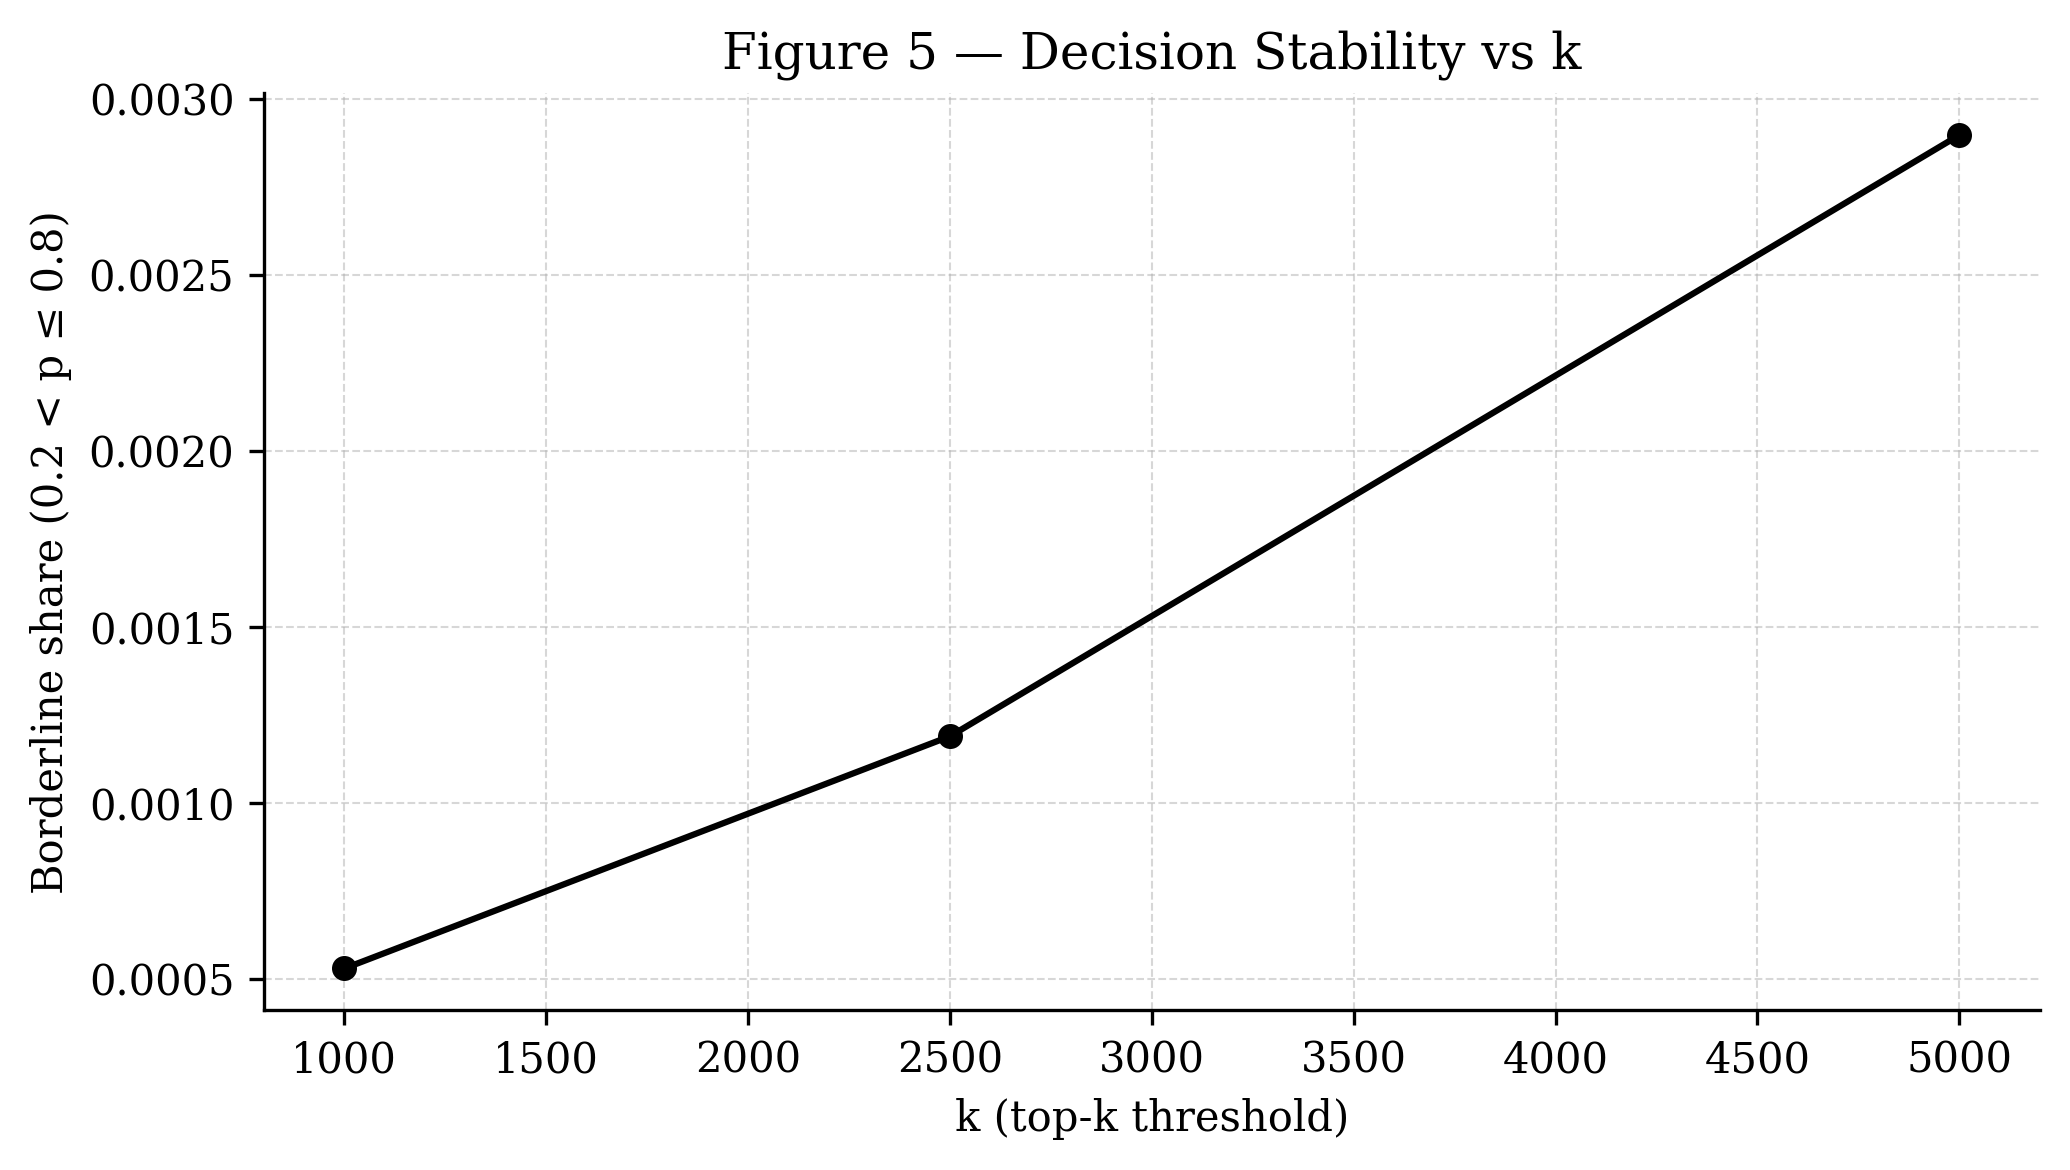
\includegraphics[keepaspectratio,alt={Decision stability as a function of prioritisation threshold (k)}]{figures/fig05_borderline_vs_k.png}}
\caption{Decision stability as a function of prioritisation threshold
(k)}
\end{figure}

Figure 6 shows the distribution of top-(k) membership probabilities for
borderline assets in the Top-1000 setting. This preliminary result
illustrates the core inferential logic of the project: the posterior
does not only produce expected risks, but also reveals where
prioritisation membership is robust and where it remains uncertain.

\begin{figure}
\centering
\pandocbounded{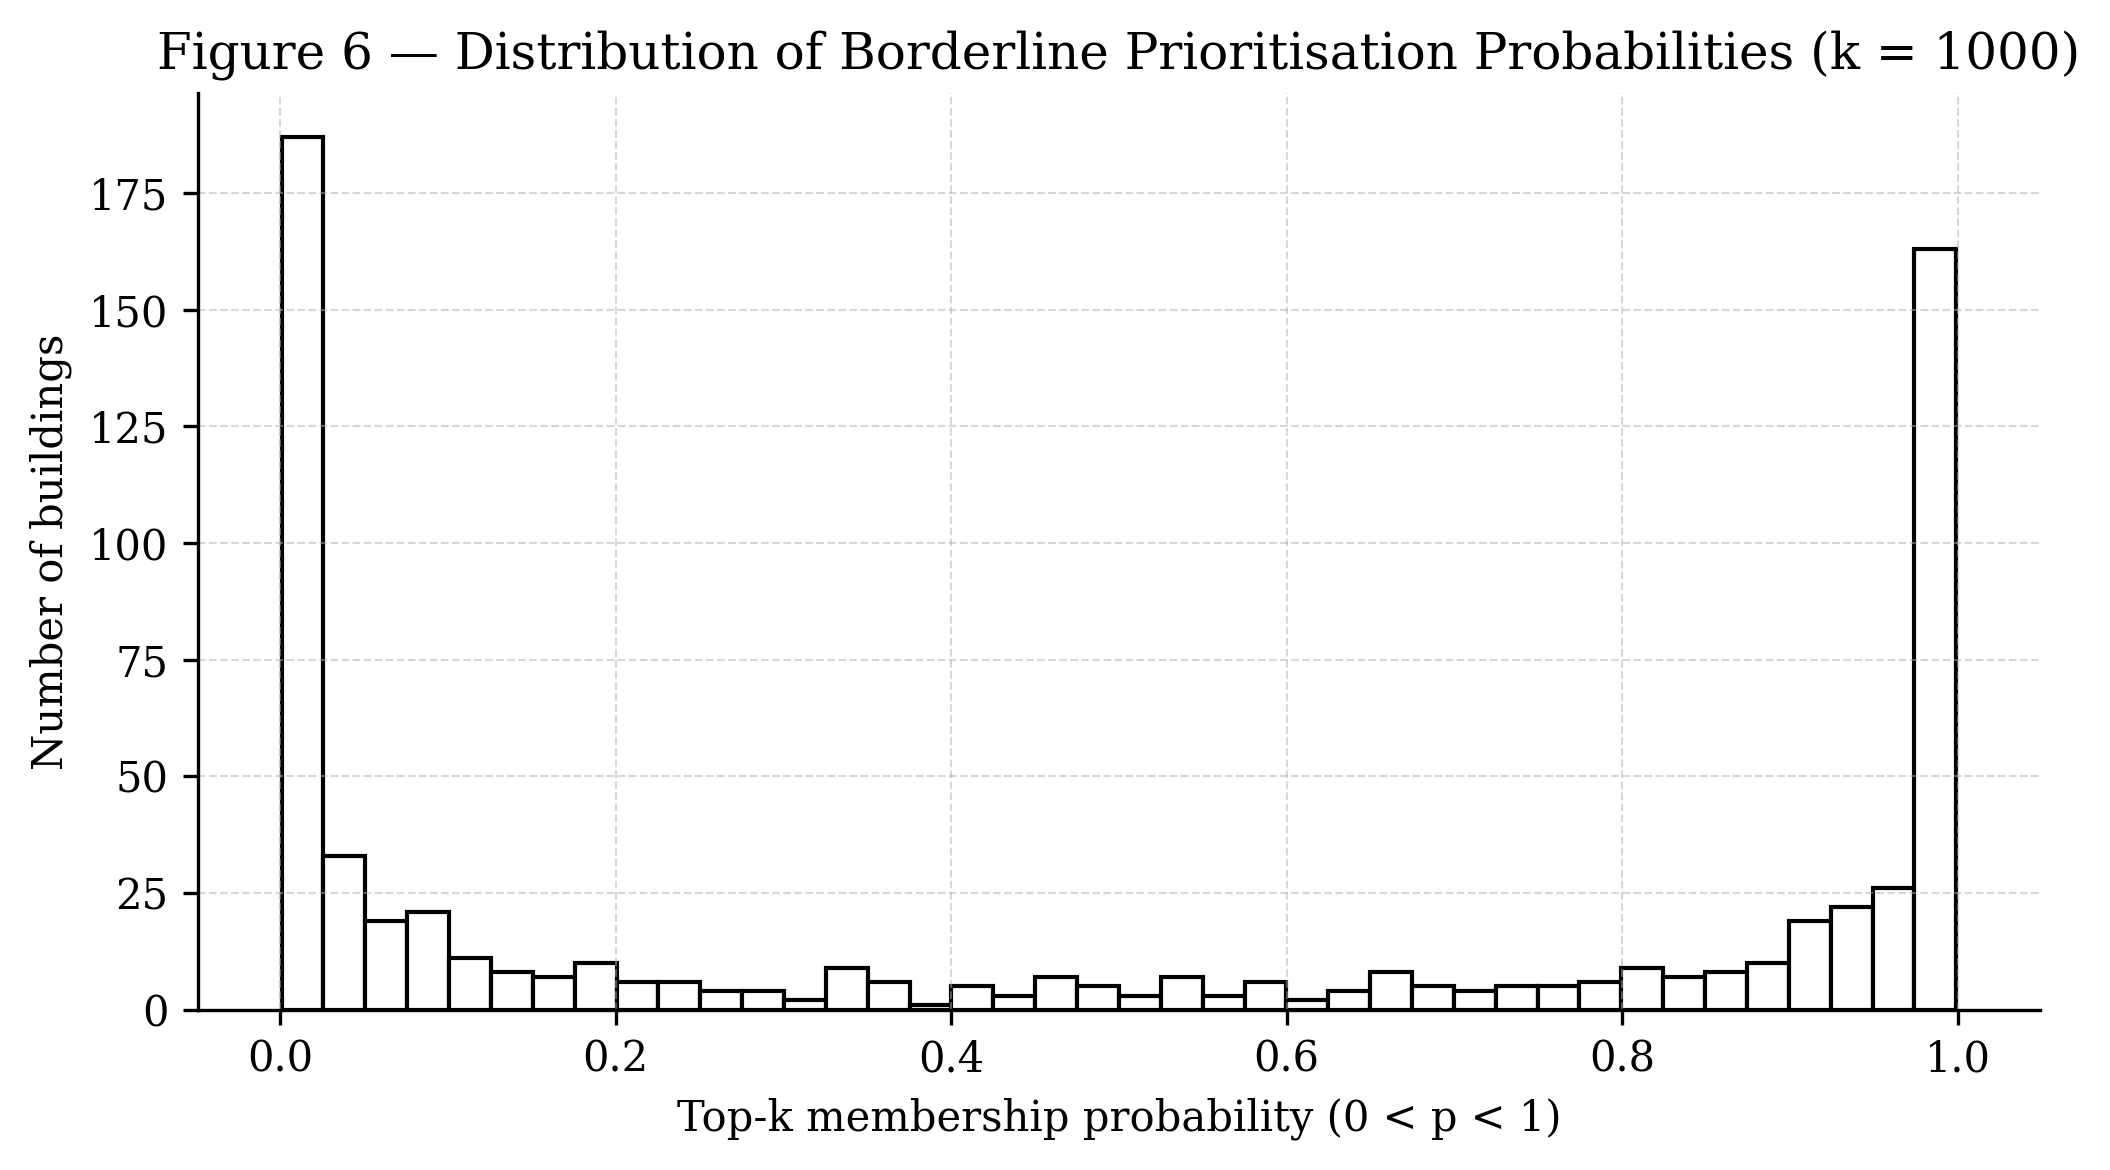
\includegraphics[keepaspectratio,alt={Distribution of borderline prioritisation probabilities for (k = 1000)}]{figures/fig06_topk_prob_histogram.png}}
\caption{Distribution of borderline prioritisation probabilities for (k
= 1000)}
\end{figure}

The work completed so far should nevertheless be understood as
foundational rather than conclusive. The current implementation relies
on a simplified hazard representation and a synthetic outcome variable,
and therefore serves primarily to validate the probabilistic inference
and decision pipeline. The next phases extend this baseline toward
richer uncertainty structures, sensitivity analysis, and cross-city
structural transfer.

\section{8. Generative Model}\label{generative-model}

The framework is formalised as a hierarchical generative model linking
exposure, hazard, and impact at the asset level.

\subsection{8.1 Generative structure}\label{generative-structure}

For each asset (i), the model defines:

\begin{itemize}
\tightlist
\item
  exposure indicators (X\_i),
\item
  hazard intensity (H\_i),
\item
  impact outcome (Y\_i),
\item
  parameter vectors (\theta\_H) and (\theta\_Y).
\end{itemize}

The generative process is specified as:

\[
H_i \sim p(H \mid X_i, \theta_H)
\]

\[
Y_i \sim p(Y \mid H_i, X_i, \theta_Y)
\]

This structure encodes the assumption that hazard conditions depend on
exposure context and that impact arises from the interaction between
hazard and exposure.

\subsection{8.2 Hazard representation}\label{hazard-representation}

Hazard is treated as a probabilistic input variable informed by
long-term precipitation patterns rather than as a hydrodynamic
simulation.

In the current implementation, (H\_i) is approximated by an observed
precipitation-derived proxy. Explicit latent hazard modelling is
reserved for later stages of the project.

\subsection{8.3 Joint posterior}\label{joint-posterior}

Given observed data, Bayesian inference yields a joint posterior:

\[
p(\theta_H, \theta_Y, H \mid \text{data})
\propto
p(Y \mid H, X, \theta_Y)\, p(H \mid X, \theta_H)\, p(\theta_H)\, p(\theta_Y)
\]

This posterior defines a distribution over plausible system states
consistent with the data and modelling assumptions.

\subsection{8.4 Posterior predictive
quantities}\label{posterior-predictive-quantities}

Posterior predictive outcomes are obtained by integrating over this
joint distribution and form the basis for downstream analysis.

\subsection{8.5 Link to decision
inference}\label{link-to-decision-inference}

Decision-level quantities are derived from posterior draws rather than
point estimates. For each posterior sample, asset-level risks are
computed and transformed into a ranking, ensuring that uncertainty
propagates coherently into prioritisation outputs.

\begin{figure}
\centering
\pandocbounded{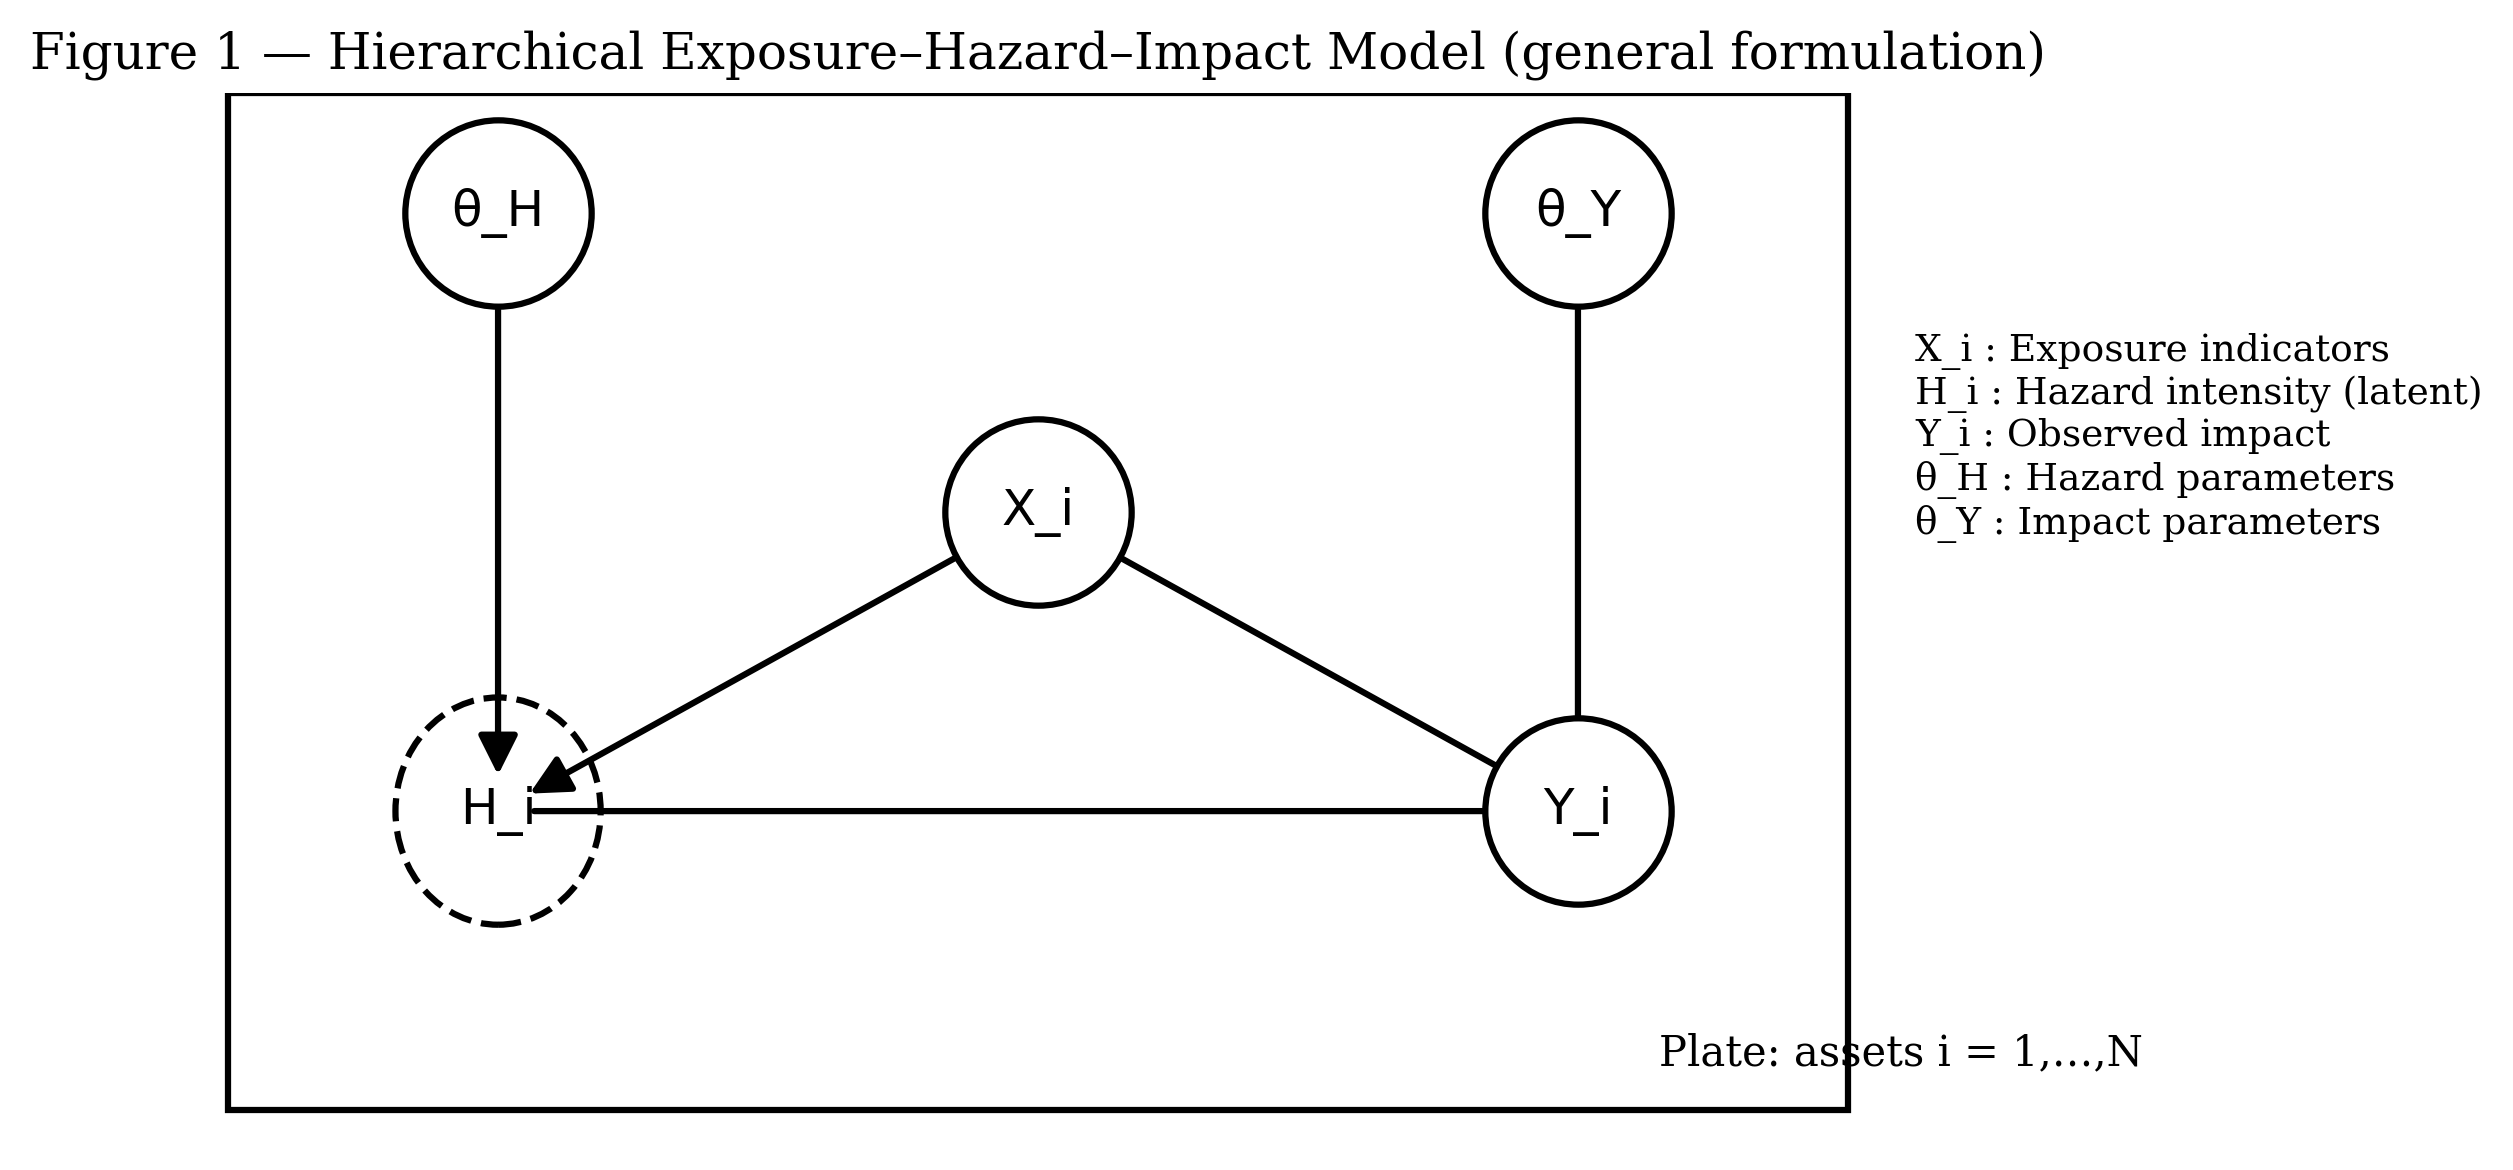
\includegraphics[keepaspectratio,alt={Hierarchical exposure--hazard--impact model}]{figures/fig01_graphical_model.png}}
\caption{Hierarchical exposure--hazard--impact model}
\end{figure}

\section{9. Model Specification}\label{model-specification}

The generative structure is instantiated as a hierarchical regression
model linking exposure, hazard, and impact.

\subsection{9.1 Baseline specification (Phase
1)}\label{baseline-specification-phase-1}

In Phase 1, the outcome (Y\_i) is defined as a binary synthetic
indicator and modelled using logistic regression:

\[
\text{logit}(p_i) = \alpha + \beta_E X_i + \beta_H H_i
\]

\[
Y_i \sim \text{Bernoulli}(p_i)
\]

where (p\_i = P(Y\_i = 1)).

Weakly informative priors are assigned to regularise inference:

\[
\alpha, \beta_E, \beta_H \sim \mathcal{N}(0, 2.5)
\]

This specification is intentionally simple and serves to validate the
probabilistic pipeline and decision-level inference.

\subsection{9.2 Predictors}\label{predictors}

Hazard enters as a continuous predictor and may interact with exposure
in extended formulations. In Phase 1, both are standardised covariates.

The hazard component is treated as an observed proxy derived from
precipitation data.

\subsection{9.3 Likelihood extensions}\label{likelihood-extensions}

The framework supports alternative likelihoods depending on data
availability:

\begin{itemize}
\tightlist
\item
  Gaussian (continuous loss ratios)
\item
  Log-normal or Gamma (positive loss values)
\item
  Zero-inflated variants (excess non-damage cases)
\end{itemize}

\subsection{9.4 Hierarchical structure and
transfer}\label{hierarchical-structure-and-transfer}

The model supports hierarchical extensions with partial pooling across
cities while maintaining a fixed structural specification. This enables
evaluation of model behaviour under domain shift without structural
redefinition.

\subsection{9.5 Inference}\label{inference}

Posterior inference is performed via MCMC. Posterior draws are
propagated directly to decision-level quantities to preserve uncertainty
required for stability analysis.

\section{10. Decision-Level Inference}\label{decision-level-inference}

The central contribution of the framework lies in deriving decision
outputs from posterior distributions rather than point estimates. While
conceptually straightforward, this step is rarely implemented in
practice because prioritisation is typically derived after uncertainty
has been collapsed into point estimates.

\subsection{10.1 Posterior-induced
rankings}\label{posterior-induced-rankings}

For each posterior sample (s), asset-level risks are computed and
converted into rankings:

\[
\text{rank}^{(s)} = \text{argsort}(\text{risk}^{(s)})
\]

Prioritisation is therefore represented as a distribution over rankings.

\subsection{10.2 Decision-level
quantities}\label{decision-level-quantities}

This enables direct computation of:

\begin{itemize}
\tightlist
\item
  posterior rank distributions (r\_i\^{}\{(s)\});
\item
  top-(k) membership probabilities, \[
  P(i \in \text{top-}k) = \frac{1}{S} \sum_{s=1}^{S} \mathbf{1}(i \in \text{top-}k^{(s)})
  \]
\item
  ranking variability measures, such as the standard deviation of ranks.
\end{itemize}

These quantities constitute the primary inferential outputs.

\subsection{10.3 Interpretation}\label{interpretation-1}

\begin{itemize}
\tightlist
\item
  High top-(k) probability indicates robust prioritisation.
\item
  Low probability indicates consistent exclusion.
\item
  Intermediate values identify assets near decision boundaries.
\end{itemize}

Similarly, concentrated rank distributions indicate stability, while
wide distributions indicate sensitivity to uncertainty.

\subsection{10.4 Inferential shift}\label{inferential-shift}

The framework shifts the question from:

\begin{quote}
Which assets have the highest expected risk?
\end{quote}

to:

\begin{quote}
Which prioritisation decisions remain stable under uncertainty?
\end{quote}

\begin{figure}
\centering
\pandocbounded{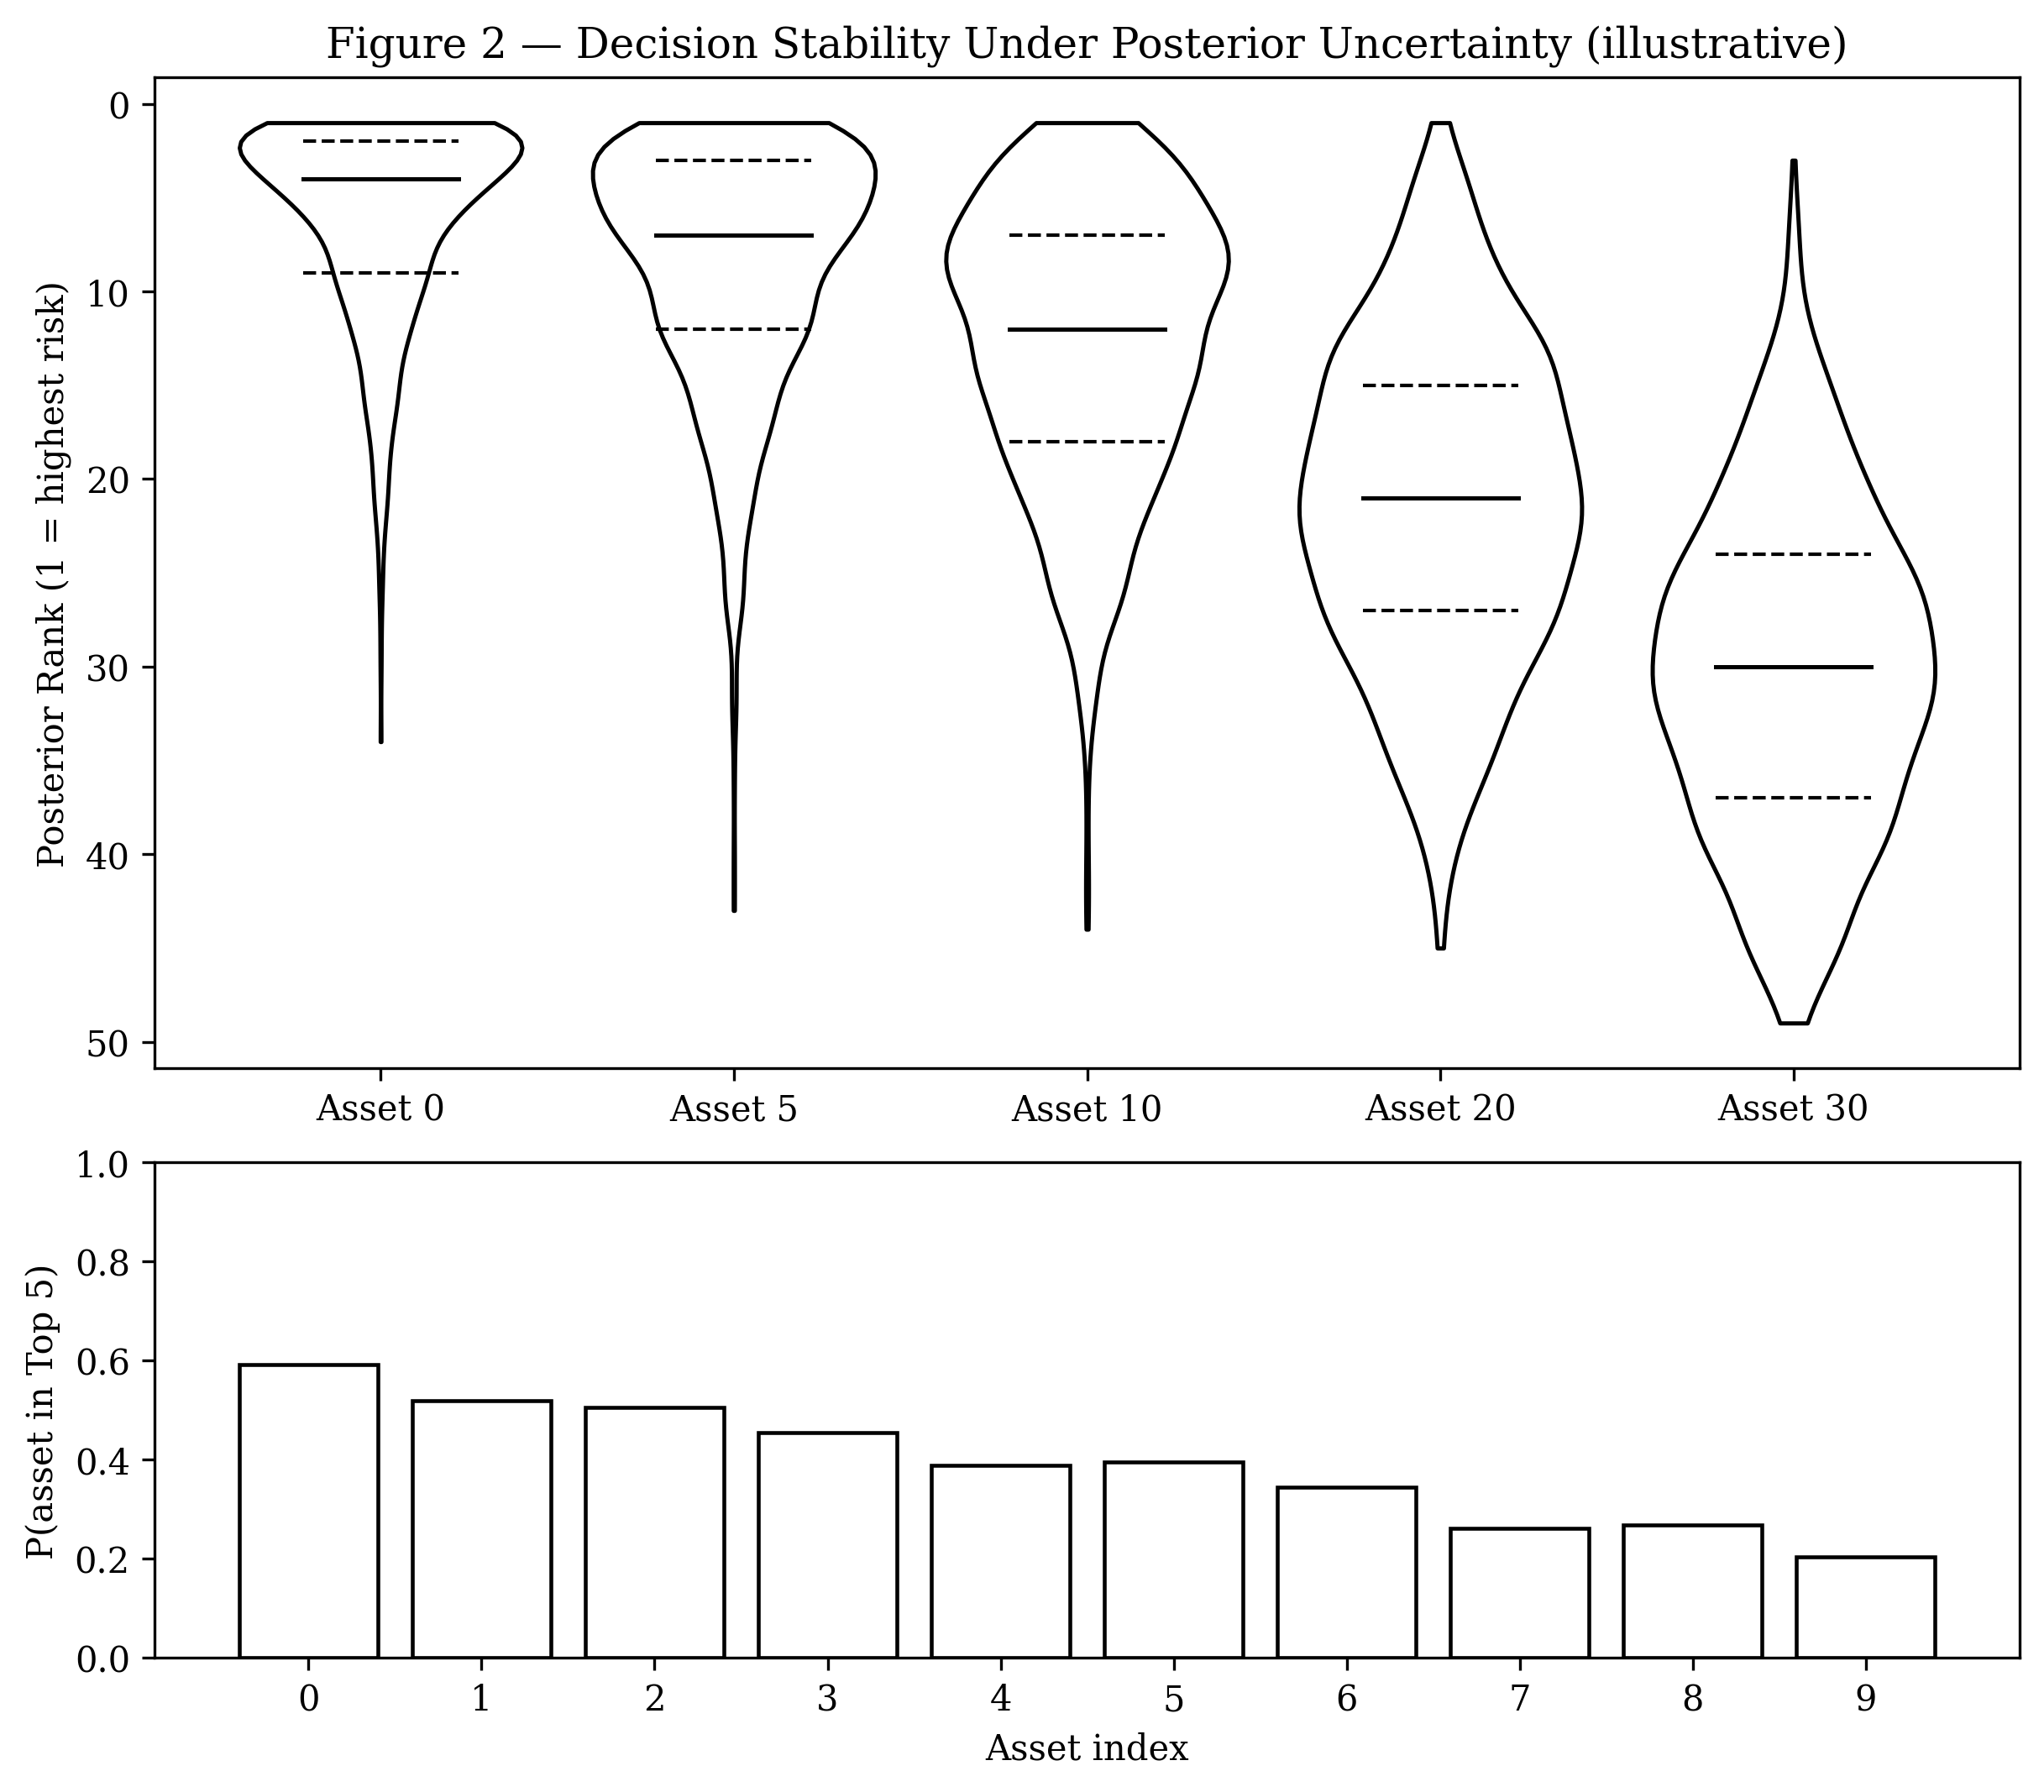
\includegraphics[keepaspectratio,alt={Decision stability concept}]{figures/fig02_decision_stability_concept.png}}
\caption{Decision stability concept}
\end{figure}

\section{11. Cross-City Transfer as Structural Stress
Test}\label{cross-city-transfer-as-structural-stress-test}

The framework is evaluated across multiple cities using an identical
generative specification.

\subsection{11.1 Transfer logic}\label{transfer-logic}

No structural modifications are introduced between contexts. Transfer is
therefore treated as a test of whether the model structure remains
informative across contexts rather than recalibration.

\subsection{11.2 Evaluation}\label{evaluation}

Analysis focuses on decision-level quantities:

\begin{itemize}
\tightlist
\item
  posterior rank distributions,
\item
  top-(k) membership probabilities,
\item
  ranking variability measures.
\end{itemize}

\subsection{11.3 Interpretation}\label{interpretation-2}

\begin{itemize}
\tightlist
\item
  Stable ranking behaviour suggests generalisable structure.
\item
  Increased variability indicates sensitivity to domain shift.
\item
  Shifts in top-(k) membership reflect changing decision boundaries.
\end{itemize}

Increases in rank dispersion are interpreted as structural stress rather
than performance failure.

\subsection{11.4 Role in the framework}\label{role-in-the-framework}

Transfer serves as a diagnostic tool for assessing whether the assumed
generative structure remains informative across contexts.

\begin{figure}
\centering
\pandocbounded{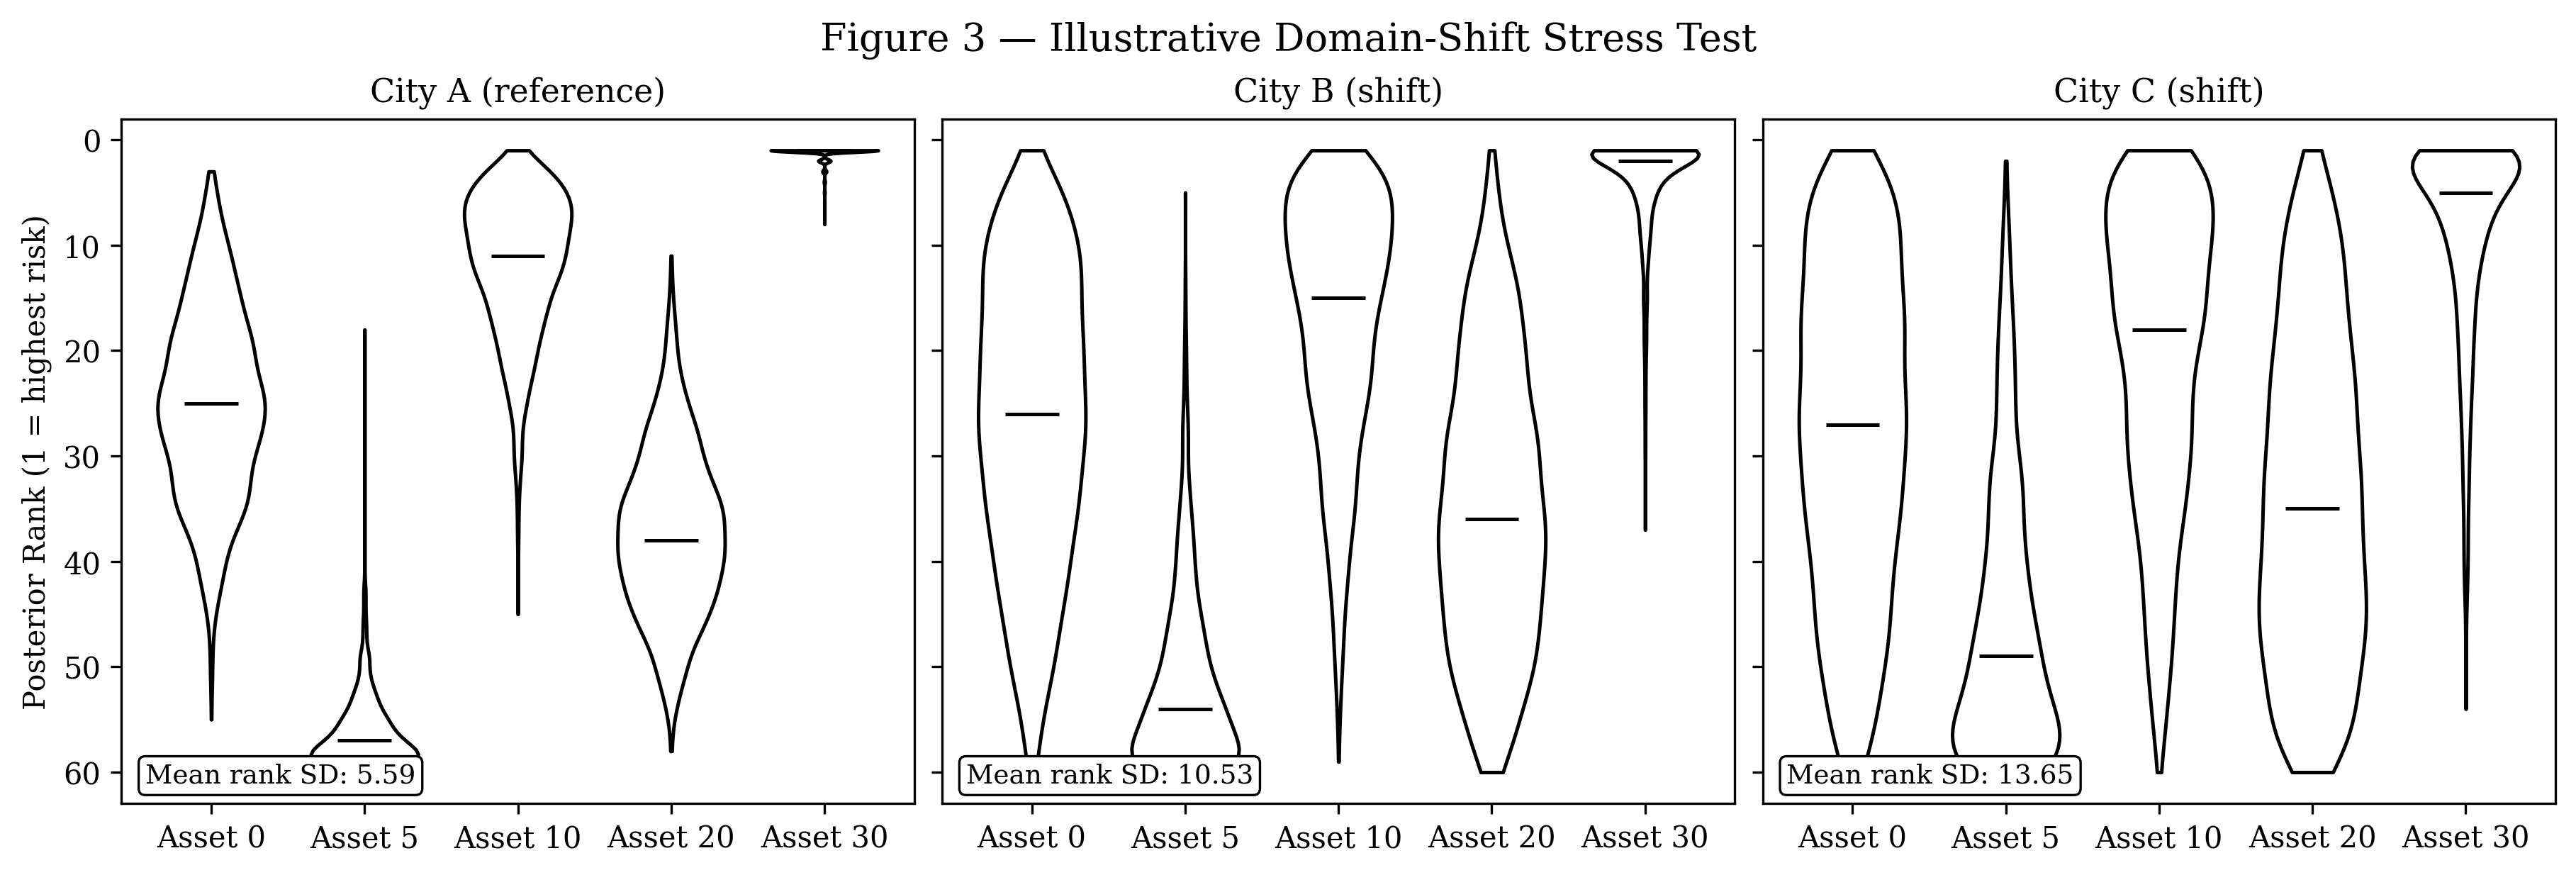
\includegraphics[keepaspectratio,alt={Domain-shift stress test concept}]{figures/fig03_domain_shift_illustrative.png}}
\caption{Domain-shift stress test concept}
\end{figure}

\section{12. Empirical Implementation}\label{empirical-implementation}

\subsection{12.1 Data and study area}\label{data-and-study-area}

The empirical analysis focuses on the municipality of Rotterdam,
comprising approximately 221,000 buildings. This scale is important
because the project is concerned with prioritisation under budget
constraints in realistic urban settings, where decisions are made over
very large asset populations rather than small illustrative samples.

The Rotterdam dataset builds on a pre-existing spatial data integration
pipeline developed prior to the present modelling work. This pipeline
combines multiple open data sources into a consistent asset-level
representation.

The dataset integrates:

\begin{itemize}
\tightlist
\item
  building geometries derived from OpenStreetMap;
\item
  hydrography layers describing relevant surface-water structures;
\item
  ERA5-Land precipitation data;
\item
  derived exposure indicators, including distance to water bodies and
  local hydrographic density at multiple spatial scales.
\end{itemize}

All data are harmonised and aggregated at the building level. The
resulting dataset provides a large-scale asset-level representation
suitable for probabilistic inference and decision analysis.

\subsection{12.2 Hazard and outcome
representation}\label{hazard-and-outcome-representation}

In Phase 1, hazard is represented by a precipitation-derived proxy
constructed from ERA5-Land indicators and standardised prior to
modelling. This representation is intentionally simplified and is used
to validate the end-to-end inference structure before introducing richer
hazard formulations.

The outcome variable is a synthetic binary indicator. It is used solely
to validate the probabilistic modelling and decision pipeline and is not
interpreted as a calibrated estimate of observed flood damage. No
empirical calibration claims are made at this stage.

\subsection{12.3 Computational workflow}\label{computational-workflow}

The modelling workflow follows the structure defined in previous
sections:

\begin{enumerate}
\def\labelenumi{\arabic{enumi}.}
\tightlist
\item
  construction of exposure and hazard covariates at the asset level;
\item
  specification of the probabilistic exposure--hazard--impact model;
\item
  Bayesian inference via MCMC;
\item
  posterior predictive evaluation of asset-level impact probabilities;
\item
  computation of posterior-derived prioritisation metrics.
\end{enumerate}

Inference is performed using Hamiltonian Monte Carlo as implemented in
PyMC. Posterior outputs are then propagated to decision-level quantities
such as rank distributions, top-(k) membership probabilities, and
related stability measures.

A first citywide output of the Phase-1 model is the distribution of
posterior mean impact probabilities across all buildings. Figure 4 shows
that these probabilities are concentrated near low values, with only a
relatively small fraction of assets occupying the upper tail of the
distribution.

\begin{figure}
\centering
\pandocbounded{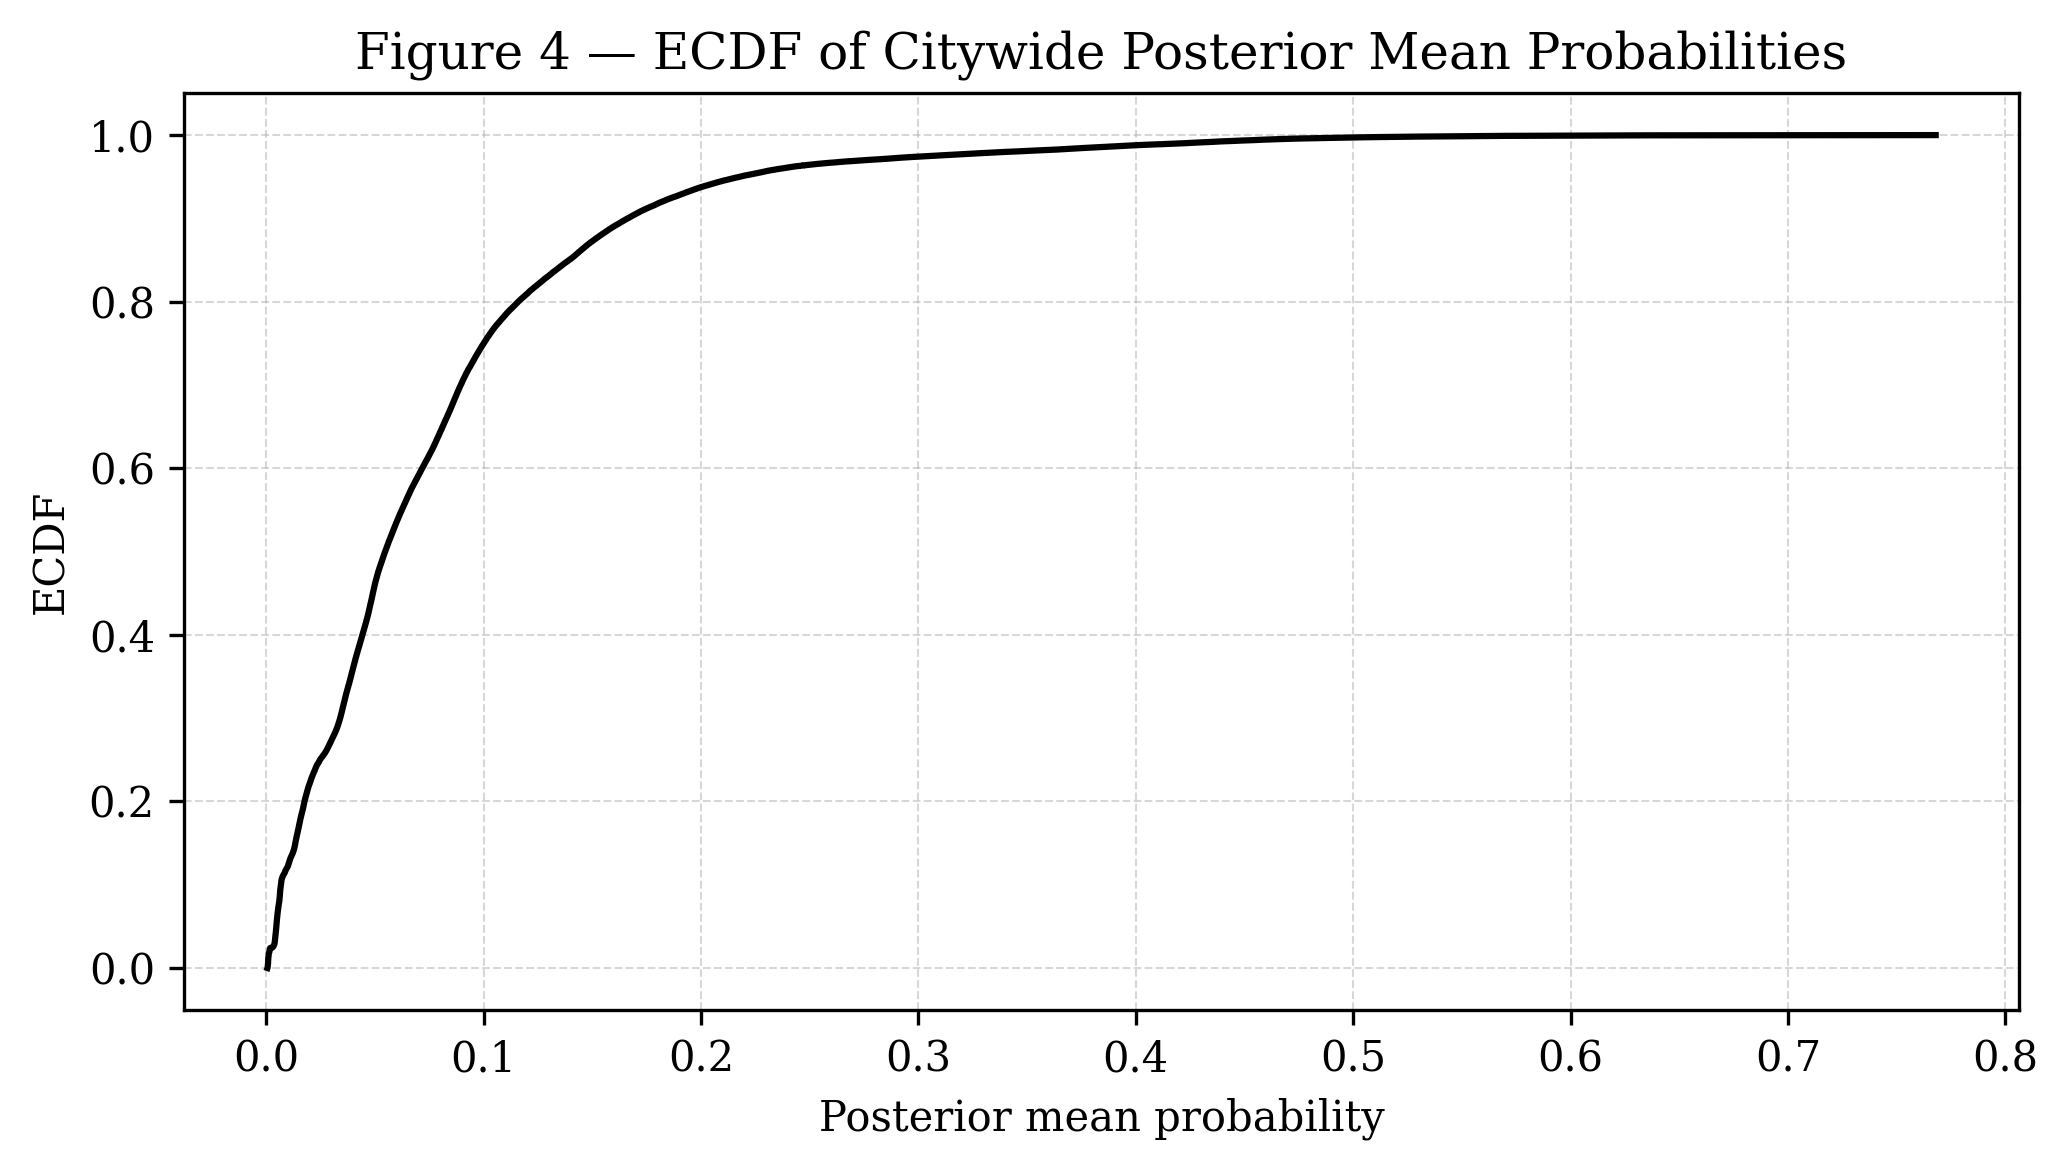
\includegraphics[keepaspectratio,alt={Empirical cumulative distribution of citywide posterior mean probabilities}]{figures/fig04_pmean_city_ecdf.png}}
\caption{Empirical cumulative distribution of citywide posterior mean
probabilities}
\end{figure}

\subsection{12.4 Reproducibility}\label{reproducibility}

All data processing, modelling, and analysis steps are implemented in
reproducible Python pipelines and maintained in open repositories. This
includes spatial preprocessing scripts, model specification and
inference code, posterior analysis workflows, and figure-generation
routines.

This reproducible computational setup is central to the project's
methodological contribution: the framework is intended not only as a
conceptual proposal, but as an operational research pipeline that can be
extended to additional cities and more complex hazard representations.

\section{13. Expected Contributions}\label{expected-contributions}

The project is primarily methodological, with empirical components
serving to demonstrate the framework in practice. Taken together, the
proposed contributions establish decision stability as a measurable
property of probabilistic risk models.

\subsection{13.1 Methodological
contributions}\label{methodological-contributions}

\begin{enumerate}
\def\labelenumi{\arabic{enumi}.}
\item
  \textbf{Unified probabilistic exposure--hazard--impact structure}\\
  Formalisation of the full risk chain within a single hierarchical
  posterior.
\item
  \textbf{Decision stability as an inferential target}\\
  Prioritisation rankings and top-(k) membership are treated as
  posterior quantities rather than deterministic outputs.
\item
  \textbf{Posterior-based ranking analysis}\\
  Explicit derivation of rank distributions and decision-level stability
  metrics from posterior draws.
\item
  \textbf{Cross-city transfer as structural stress test}\\
  Evaluation of whether the same generative structure remains
  informative under domain shift.
\end{enumerate}

\subsection{13.2 Empirical contributions}\label{empirical-contributions}

\begin{enumerate}
\def\labelenumi{\arabic{enumi}.}
\item
  \textbf{Quantification of prioritisation instability}\\
  Measurement of how epistemic uncertainty affects ranking behaviour in
  a large urban asset population.
\item
  \textbf{Evidence on decision boundaries}\\
  Identification of narrow subsets of assets for which prioritisation
  membership is sensitive to uncertainty.
\item
  \textbf{Evidence under domain shift}\\
  Analysis of how ranking behaviour changes across cities when the
  generative specification is held fixed.
\end{enumerate}

The project therefore reframes flood risk modelling from expected-loss
estimation toward decision stability analysis.

\section{14. Limitations and Scope}\label{limitations-and-scope}

The current implementation adopts a simplified specification to isolate
the behaviour of the inference and decision pipeline.

\subsection{14.1 Hazard}\label{hazard}

Hazard is represented by a precipitation proxy rather than a
hydrodynamic model. Detailed flood processes are not captured.

\subsection{14.2 Outcome}\label{outcome}

The outcome variable is synthetic and not calibrated to observed damage.

\subsection{14.3 Exposure}\label{exposure}

Exposure is approximated using hydrography-based indicators and does not
capture the full range of vulnerability factors (e.g.~building typology,
elevation, drainage conditions).

\subsection{14.4 Scope}\label{scope-1}

Results should be interpreted as evidence about the probabilistic
framework rather than operational risk estimates. Future work will
extend hazard, outcome, and exposure representations while preserving
the generative structure.

\section{15. Work Plan}\label{work-plan}

The project is structured in four phases. Preparatory work conducted
prior to the formal project start (November 2025 -- January 2026)
established the spatial data pipeline and initial exposure indicators
that enable the Phase 1 implementation.

\subsection{Phase 1 --- Baseline probabilistic pipeline
(completed)}\label{phase-1-baseline-probabilistic-pipeline-completed}

February--March 2026

\textbf{Tasks} - Finalisation of the Rotterdam exposure--hazard--impact
dataset building on the pre-existing spatial data pipeline -
Implementation of the Bayesian baseline model - Computation of posterior
decision stability metrics - Preparation of a methodological baseline
manuscript (working paper / preprint)

\textbf{Expected output} - city-scale Rotterdam dataset ready for
probabilistic modelling; - baseline Bayesian workflow implemented; -
initial decision-stability results and figures; - methodological draft
documenting the framework.

\textbf{Risk} - Limited empirical realism due to simplified hazard and
synthetic outcome representation.

\textbf{Mitigation} - Treat Phase 1 explicitly as methodological
validation of the inference and decision pipeline rather than as a final
operational model.

\subsection{Phase 2 --- Posterior decision stability
analysis}\label{phase-2-posterior-decision-stability-analysis}

April--June 2026

\textbf{Tasks} - Extension of posterior analysis - Sensitivity analysis
of priors and model specifications - Evaluation of alternative hazard
proxy definitions - Robustness analysis of ranking-based decision
metrics

\textbf{Expected output} - refined posterior decision-stability
analysis; - sensitivity results for model assumptions and ranking
metrics; - clearer characterisation of decision boundaries under
uncertainty.

\textbf{Risk} - Posterior ranking behaviour may prove highly sensitive
to modelling choices, making interpretation unstable.

\textbf{Mitigation} - compare multiple specifications explicitly and
treat sensitivity itself as a substantive result rather than a failure.

\subsection{Phase 3 --- Cross-city structural
transfer}\label{phase-3-cross-city-structural-transfer}

July--October 2026

\textbf{Tasks} - Application of the fixed-specification model to
additional cities - Evaluation of posterior ranking behaviour under
domain shift - Quantification of instability changes across contexts

\textbf{Expected output} - comparative transfer analysis across urban
contexts; - empirical evidence on whether the same generative structure
remains informative under domain shift; - assessment of structural
stress through changes in decision-level quantities.

\textbf{Risk} - transfer may reveal strong context dependence and
degraded ranking stability.

\textbf{Mitigation} - interpret instability inflation as evidence about
structural limits of the model, not simply as predictive failure.

\subsection{Phase 4 --- Model extension and
synthesis}\label{phase-4-model-extension-and-synthesis}

November 2026 -- February 2027

\textbf{Tasks} - Introduction of an explicit latent hazard layer -
Comparison of proxy-based and latent hazard formulations - Integration
of cross-city results - Preparation of journal manuscript

\textbf{Expected output} - extended model specification with richer
hazard treatment; - synthesis of within-city and cross-city findings; -
journal manuscript presenting the research programme and results.

\textbf{Risk} - increasing model complexity may reduce interpretability
or make inference computationally more demanding.

\textbf{Mitigation} - retain the simplest defensible specification as
baseline and introduce additional complexity only where it improves
inferential value.

\section{16. References}\label{references}

Gelman, A., Carlin, J. B., Stern, H. S., Dunson, D. B., Vehtari, A., \&
Rubin, D. B. (2013). \emph{Bayesian data analysis} (3rd ed.). CRC Press.

Hall, J. W., \& Harvey, H. (2009). Decision making under severe
uncertainties for flood risk management: A case study of Info-Gap
robustness analysis. In \emph{Proceedings of the 8th International
Conference on Hydroinformatics}, Concepción, Chile.

Lv, H., Wu, Z., Guan, X., \& Meng, Y. (2021). The construction of flood
loss ratio function in cities lacking loss data based on dynamic
proportional substitution and hierarchical Bayesian model. \emph{Journal
of Hydrology, 592}, 125797.
https://doi.org/10.1016/j.jhydrol.2020.125797

Matrosov, E. S., Woods, A. M., \& Harou, J. J. (2013). Robust decision
making and Info-Gap decision theory for water resource system planning.
\emph{Journal of Hydrology, 494}, 43--58.
https://doi.org/10.1016/j.jhydrol.2013.03.006

McElreath, R. (2020). \emph{Statistical rethinking: A Bayesian course
with examples in R and Stan} (2nd ed.). Chapman and Hall/CRC.

McMillan, H. K., \& Brasington, J. (2008). End-to-end flood risk
assessment: A coupled model cascade with uncertainty estimation.
\emph{Water Resources Research, 44}(3).
https://doi.org/10.1029/2007WR005995

Mohor, G. S., Thieken, A. H., \& Korup, O. (2021). Residential flood
loss estimated from Bayesian multilevel models. \emph{Natural Hazards
and Earth System Sciences, 21}, 1599--1614.
https://doi.org/10.5194/nhess-21-1599-2021

Raiffa, H., \& Schlaifer, R. (1961). \emph{Applied statistical decision
theory}. Harvard University Press.

Sairam, N., Schröter, K., Rözer, V., Merz, B., \& Kreibich, H. (2019). A
Bayesian hierarchical model for flood damage estimation in data-scarce
regions. \emph{Water Resources Research, 55}(11), 9129--9151.
https://doi.org/10.1029/2019WR025068

Vehtari, A., Gelman, A., \& Gabry, J. (2017). Practical Bayesian model
evaluation using leave-one-out cross-validation and WAIC.
\emph{Statistics and Computing, 27}, 1413--1432.
https://doi.org/10.1007/s11222-016-9696-4

Wu, Z., Shen, Y., Wang, H., \& Wu, M. (2019). Assessing urban flood
disaster risk using Bayesian network model and GIS applications.
\emph{International Journal of River Basin Management, 17}(4),
2163--2184. https://doi.org/10.1080/19475705.2019.1685010

Wu, Z., Shen, Y., Wang, H., \& Wu, M. (2020). Urban flood disaster risk
evaluation based on ontology and Bayesian network. \emph{Journal of
Hydrology, 583}, 124596. https://doi.org/10.1016/j.jhydrol.2020.124596

\end{document}
